% Generated by scripts/generate_relative_origin_share.py. Do not edit.
% The x-axis is the geometric mean of AU and NZ decision shares. The y-axis is
% log2(AU share / NZ share). Labels show the three largest average shares, the
% largest positive and negative ratios among origins with geometric-mean share
% at least 0.1%, the most negative ratio overall, and the upper and lower
% ratio boundaries among origins with geometric-mean share below 0.01%, the
% lower boundary below 0.001%, the upper boundary from 0.01% to 0.1%, and the
% origin with the smallest geometric-mean share.
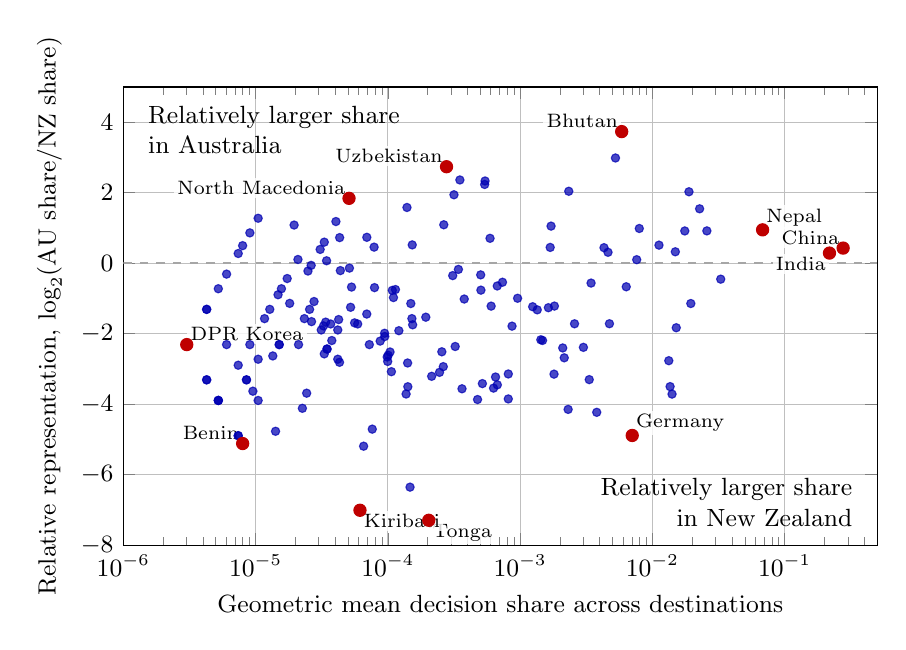
\begin{tikzpicture}
\begin{semilogxaxis}[
  width=0.92\textwidth,height=7.4cm,xmin=0.000001,xmax=0.5,ymin=-8,ymax=5,
  xlabel={Geometric mean decision share across destinations},
  ylabel={Relative representation, $\log_2(\mathrm{AU\ share}/\mathrm{NZ\ share})$},
  grid=major,tick label style={font=\small},label style={font=\small},
]
\addplot[gray!70,dashed,thick,domain=0.000001:0.5,forget plot] {0};
\addplot[only marks,mark=*,mark size=1.5pt,blue!70!black,opacity=0.72] coordinates {(0.000141653966367,-3.50519430713) (4.37550682435e-05,-0.210107824465) (3.46901105437e-05,-2.4351743801) (5.2297309368e-06,-3.89460599874) (0.000672788167152,-3.45151221433) (2.48984994571e-05,-0.222180656766) (0.000476757218423,-3.86823058331) (4.32310365463e-05,0.725980411715) (7.98854596071e-06,0.497711424041) (2.63224018092e-05,-0.0617159845726) (0.0227511072134,1.54366133588) (1.28101722872e-05,-1.30964349802) (3.46901105437e-05,-2.4351743801) (0.000363682573553,-3.56340009026) (1.04594618736e-05,-2.7246809973) (7.98854596071e-06,-5.11699842007) (4.27005742907e-06,-3.30964349802) (0.00586090465273,3.73392724357) (0.000106409282809,-3.07831795191) (9.05815969244e-06,0.860281503426) (0.000139546626609,1.58112743223) (0.00379622514813,-4.2310515294) (0.000264864058994,1.09028710887) (4.18378474944e-05,-1.89460599874) (3.07918220193e-05,0.390796220125) (4.27005742907e-06,-1.30964349802) (0.00461783267486,0.309592564005) (9.48106612709e-05,-2.08016165189) (0.00634508838478,-0.668797070514) (2.25950200825e-05,-4.11699842007) (0.00230697731626,-4.14828579265) (0.276698921953,0.428974440983) (0.0112174823151,0.512535523046) (0.000592461812698,0.705953357035) (0.00333170392898,-3.30317192979) (5.2297309368e-06,-3.89460599874) (4.18378474944e-05,-2.7246809973) (2.33880677574e-05,-1.57267790385) (0.000214440226424,-3.20911662206) (3.01938656415e-06,-2.30964349802) (5.9167651347e-05,-1.7246809973) (0.000629887748839,-3.54410875165) (7.39595641838e-06,0.275319002705) (2.09189237472e-05,0.105394001263) (2.43430727219e-05,-3.68815512127) (0.000518456017399,-3.41655870193) (0.000505492565456,-0.764482005353) (2.76731349651e-05,-1.08725107668) (1.81163193849e-05,-1.13971849657) (2.64950095722e-05,-1.65756680144) (1.50969328207e-05,-2.30964349802) (0.000152022440423,-1.57267790385) (0.00215574685597,-2.68443340729) (0.000256007659971,-2.51365739004) (0.00300922432395,-2.38780256094) (2.1135705949e-05,-2.30964349802) (0.00703969961243,-4.88803794833) (0.000735888372167,-0.540256426158) (5.2297309368e-05,-1.25074980896) (8.54011485813e-06,-3.30964349802) (6.93802210875e-05,0.734750621342) (6.0387731283e-06,-2.30964349802) (7.39595641838e-06,-4.89460599874) (1.50969328207e-05,-2.30964349802) (4.24865349764e-05,-1.59915011521) (0.000141105855189,-2.83159620121) (3.26596592325e-05,-1.77912878132) (0.218123454103,0.287010314115) (0.0175772120366,0.915047306857) (0.00343930794191,-0.563890825627) (0.000154077494666,-1.74776461041) (0.000245927135783,-3.09691417403) (9.8905075578e-05,-2.66111586852) (0.00180445422476,-3.14756416976) (3.30757226202e-05,-2.57267790385) (0.0140787219025,-3.71394426005) (0.000503468563072,-0.331273513988) (0.000378087002036,-1.01686174879) (0.00525936232302,2.98530775763) (6.15836440387e-05,-7.01008321616) (0.00163628188384,-1.26258469322) (7.93127965992e-05,-0.692972137568) (0.00143411008723,-2.17300880599) (3.7712126099e-05,-2.1941662806) (0.000350535045646,2.36155140035) (3.13783856208e-05,-1.89460599874) (1.41621783255e-05,-4.76907511665) (7.39595641838e-06,-2.89460599874) (5.31617862695e-05,-0.677375282517) (4.31254660919e-05,-2.81214383855) (1.04594618736e-05,1.2753190027) (7.87359686049e-05,0.455891248347) (0.0149093395146,0.324220515401) (0.000309453981442,-0.351871733405) (8.54011485813e-06,-3.30964349802) (1.73450552719e-05,-0.4351743801) (7.39595641838e-06,-4.89460599874) (0.000539541652878,2.23411988553) (0.00147826650004,-2.19180700772) (5.2297309368e-06,-3.89460599874) (0.00171372465682,1.05247368699) (6.93144889826e-05,-1.44291002888) (3.44263035932e-05,0.0688681252375) (0.00473401395397,-1.71754357725) (3.38925301238e-05,-1.6722135774) (5.12406891488e-05,-0.139718496574) (0.0681049885097,0.946615789339) (0.000651998758886,-3.22934186993) (6.0387731283e-06,-0.309643498016) (4.27005742907e-06,-1.30964349802) (0.00430725838328,0.440378248975) (5.08836068253e-05,1.84010362149) (0.00181702860239,-1.21642467006) (0.00060390750594,-1.2178510221) (0.018904449687,2.02676293508) (0.000103894981327,-2.51909686365) (0.00124430968141,-1.23538894332) (0.000114179131937,-0.746707303625) (0.000957197926235,-0.994910904533) (0.0195278615368,-1.1439567997) (0.000193711944756,-1.53203591935) (0.000341577905424,-0.175787751281) (0.0151538460548,-1.83121345426) (0.000110279968392,-0.975224458946) (0.00210034528155,-2.40502876385) (0.000108067046696,-0.771223583232) (1.47919128368e-05,-0.894605998737) (1.04594618736e-05,-3.89460599874) (0.000147177674433,-6.35403761737) (0.00233220787832,2.04110186929) (4.27005742907e-06,-3.30964349802) (3.30757226202e-05,0.597247097592) (1.95678613905e-05,1.08267392476) (4.05093216467e-05,1.18220959831) (0.00796326328856,0.984780795069) (0.000121152297998,-1.9153645589) (1.56891928104e-05,-0.724680997295) (0.000323017920302,-2.36358230513) (1.16940338787e-05,-1.57267790385) (0.00134718789275,-1.32336177926) (2.56203445744e-05,-1.30964349802) (0.000814227288091,-3.14328511159) (0.0328580153385,-0.452828809462) (5.60826163102e-05,-1.69297213757) (9.4521750509e-05,-1.98771540313) (9.54813867922e-06,-3.6315715929) (0.000868828155925,-1.78608154196) (0.000814003322391,-3.85135280078) (0.000100595883108,-2.61220626804) (0.00761294718517,0.0995302185157) (9.05815969244e-06,-2.30964349802) (0.0133039126569,-2.76645733307) (0.000262530409461,-2.93524798323) (5.2297309368e-06,-0.724680997295) (0.000203892447679,-7.29453660563) (3.69797820919e-05,-1.7246809973) (1.35031072156e-05,-2.6315715929) (6.55978669288e-05,-5.19228654738) (0.00067177110207,-0.646071162599) (0.000316214979427,1.94144435632) (8.75101364869e-05,-2.21010782447) (0.000543187558972,2.33260880606) (0.0025787187574,-1.71916399233) (0.000149207807223,-1.14458425175) (0.0136127669495,-3.50138146778) (7.62656643107e-05,-4.70819287451) (0.000277783563902,2.7374804141) (0.000137440141529,-3.71174194159) (9.97769070694e-05,-2.78769079482) (0.025818350606,0.916798854639) (7.24652775396e-05,-2.30964349802) (0.000152919335759,0.519244585591) (0.00168818544417,0.447975206314)};
\addplot[only marks,mark=*,mark size=2.2pt,red!75!black] coordinates {(0.276698921953,0.428974440983) (0.218123454103,0.287010314115) (0.0681049885097,0.946615789339) (0.00586090465273,3.73392724357) (0.00703969961243,-4.88803794833) (0.000203892447679,-7.29453660563) (5.08836068253e-05,1.84010362149) (6.15836440387e-05,-7.01008321616) (7.98854596071e-06,-5.11699842007) (0.000277783563902,2.7374804141) (3.01938656415e-06,-2.30964349802)};
\node[font=\small,align=left,anchor=north west] at (rel axis cs:0.02,0.98) {Relatively larger share\\in Australia};
\node[font=\small,align=right,anchor=south east] at (rel axis cs:0.98,0.02) {Relatively larger share\\in New Zealand};
\node[font=\scriptsize,anchor=south east,fill=white,fill opacity=0.82,text opacity=1,inner sep=1.2pt] at (axis cs:0.276698921953,0.428974440983) {China};
\node[font=\scriptsize,anchor=north east,fill=white,fill opacity=0.82,text opacity=1,inner sep=1.2pt] at (axis cs:0.218123454103,0.287010314115) {India};
\node[font=\scriptsize,anchor=south west,fill=white,fill opacity=0.82,text opacity=1,inner sep=1.2pt] at (axis cs:0.0681049885097,0.946615789339) {Nepal};
\node[font=\scriptsize,anchor=south east,fill=white,fill opacity=0.82,text opacity=1,inner sep=1.2pt] at (axis cs:0.00586090465273,3.73392724357) {Bhutan};
\node[font=\scriptsize,anchor=south west,fill=white,fill opacity=0.82,text opacity=1,inner sep=1.2pt] at (axis cs:0.00703969961243,-4.88803794833) {Germany};
\node[font=\scriptsize,anchor=north west,fill=white,fill opacity=0.82,text opacity=1,inner sep=1.2pt] at (axis cs:0.000203892447679,-7.29453660563) {Tonga};
\node[font=\scriptsize,anchor=south east,fill=white,fill opacity=0.82,text opacity=1,inner sep=1.2pt] at (axis cs:5.08836068253e-05,1.84010362149) {North Macedonia};
\node[font=\scriptsize,anchor=north west,fill=white,fill opacity=0.82,text opacity=1,inner sep=1.2pt] at (axis cs:6.15836440387e-05,-7.01008321616) {Kiribati};
\node[font=\scriptsize,anchor=south east,fill=white,fill opacity=0.82,text opacity=1,inner sep=1.2pt] at (axis cs:7.98854596071e-06,-5.11699842007) {Benin};
\node[font=\scriptsize,anchor=south east,fill=white,fill opacity=0.82,text opacity=1,inner sep=1.2pt] at (axis cs:0.000277783563902,2.7374804141) {Uzbekistan};
\node[font=\scriptsize,anchor=south west,fill=white,fill opacity=0.82,text opacity=1,inner sep=1.2pt] at (axis cs:3.01938656415e-06,-2.30964349802) {DPR Korea};
\end{semilogxaxis}
\end{tikzpicture}
